\section{Architektur und Implementierung} \label{s:implementation}
In Kapitel \ref{s:solution} wurden Konzepte für einen \textit{klugen} \ac{mqtt} \acl{lb} beschrieben. In diesem Kapitel wird gezeigt, wie man einige dieser Konzepte in einen Envoy \acl{lb} integriert.
Im Rahmen der Thesis wurde die \ac{dns} Cluster Discovery \ref{ss:dns-discovery}, das weighted \ac{cpu} round-robin \ref{ss:weighted-cpu}, der Überlastschutz \ref{ss:circuit-breaking} und der \ac{mqtt} Health Check \ref{ss:health-check} aus Kapitel \ref{s:solution} in einer Envoy Control Plane implementiert.

\subsection{Envoy Control Plane} \label{si:control-plane}
Die Envoy Control Plane ist die \textit{kluge} Komponente des Systems aus Kapitel \ref{s:solution}. Obwohl die einzelnen Envoy Instanzen die load balancing Entscheidung treffen, liefert die Control Plane alle Informationen, auf dessen Basis diese Entscheidung getroffen wird.
Als Quellcodebasis für die Control Plane wurde ein minimales Beispiel aus dem offiziellen Github Repository \cite{EnvoyproxyGocontrolplane} verwendet. Dieses startet einen gRPC Server der eine Envoy Konfiguration erzeugt, die einen \ac{http} Endpunkt definiert. Da die offizielle Referenzimplementierung einer Control Plane in Golang programmiert ist, wurde die Control Plane des Smart Load Balancers, nachfolgend Control Plane genannt, ebenfalls in Golang implementiert.
\\
Die parallele Ausführung von mehreren Go Routinen ist ein wichtiger Bestandteil der Control Plane. Diese muss asynchron und nicht blockend Aufgaben abarbeiten, wie zum Beispiel das Überprüfen eines Health Status der HiveMQ Nodes, und parallel den neusten Snapshot an alle Envoys ausliefern.
Um bei einem asynchronen Programm keine \textit{Data Races} zu verursachen, muss darauf geachtet werden, dass immer nur eine Go Routine Schreibzugriff auf eine Variable erhält und lesende Go Routinen sich zu Beginn eine Kopie der Variable erstellen, damit diese nicht während der Bearbeitung von der schreibenden Go Routine verändert wird.
\\
Die Control Plane besteht aus den in Abbildung \ref{fig:component-diagram} dargestellten Komponenten. Komponenten des Paketes \verb|github.com/breuerfelix/mqtt-control-plane| wurden im Rahmen der Thesis programmiert.
\begin{itemize}
  \item \textbf{Main:} Die Main Komponente ist der Einstiegspunkt des Programms und initialisiert die Metrics, Resources und Cluster Komponente. Nach der Initialisierung werden alle nötigen Go Routinen aufgerufen und anschlie{\ss}end ein gRPC Server gestartet, der eingehende Envoy Verbindungen akzeptiert, um die aktuelle Konfiguration eines Cache-Speichers auszuliefern.
  \item \textbf{Resources:} Generiert Envoy Ressourcen basierend einer Cluster Struktur. Es wird ein \ac{tcp} Listener und ein Upsteam Envoy Cluster mit allen Endpunkten und Gewichtungen erzeugt. Die Envoy Ressourcen werden als Snapshot zusammengefasst und können in einem Cache-Speicher hinterlegt werden.
  \item \textbf{Metrics:} Wertet periodisch alle Metriken der HiveMQ Nodes einer Cluster Struktur aus. Dabei werden Health Status und Gewichtung entsprechend angepasst.
  \item \textbf{Cluster:} Ein Cluster repräsentiert ein HiveMQ Cluster und dient als Container für eine Liste von allen HiveMQ Node Strukturen. Ein Cluster enthält zudem einen Domainnamen, unter dem die \ac{dns} Discovery die einzelnen Nodes entdecken kann.
  \item \textbf{Node:} Node ist eine Struktur, die alle Daten eines HiveMQ Nodes enthält. Darunter befinden sich \ac{ip} Adresse, Port, Health Status, Weight und nach Zeitstempel sortierte Metriken für einen bestimmten Zeitraum.
\end{itemize}
\begin{figure}
    \centering
    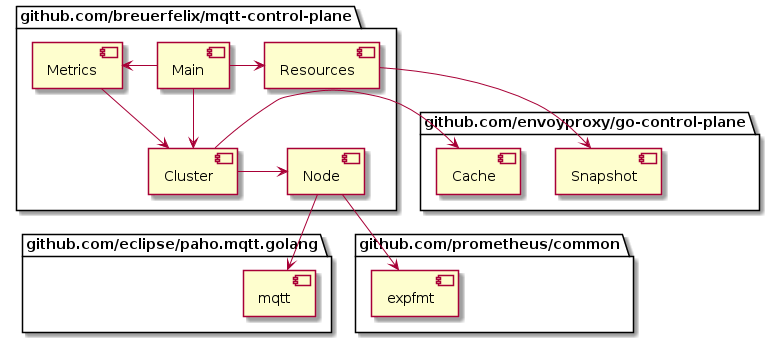
\includegraphics[scale=0.5]{gen/component-diagram.png}
    \caption{Die Abbildung zeigt das UML Komponentendiagramm der entwickelten Control Plane. Die Komponenten des Paketes \textit{github.com/breuerfelix/mqtt-control-plane} wurden im Rahmen der vorliegenden Thesis programmiert.}
    \label{fig:component-diagram}
\end{figure}
Abbildung \ref{fig:class-diagram} zeigt die Cluster und Node Strukturen in einem UML Klassendiagramm.
\begin{itemize}
  \item \textbf{Cluster:} Die Cluster Struktur enthält alle Daten um die Envoy Konfiguration für ein HiveMQ Cluster zu generieren. Die Funktion \verb|CheckNodes| löst die \ac{ip} Adressen der Domain des Feldes \verb|Domain| auf. Anhand der erhaltenen \ac{ip} Adressen wird die Liste aller Node Strukturen des Clusters erstellt. Die Funktion \verb|UpdateSnapshot| benutzt die Resources Komponente um einen Snapshot des aktuellen Clusters zu bilden und in den Cache-Speicher des \verb|Cache| Feldes zu speichern.
  \item \textbf{Node:} Eine Node Struktur repräsentiert einen HiveMQ Node. Die Funktion\newline \verb|FetchMetrics| ruft die aktuellen Prometheus Metriken des Nodes ab und speichert die geparsten Daten in dem \verb|Metrics| Feld der Struktur ab. Die Funktion \verb|filterOldData| löscht alte gespeicherte Metriken, die nicht mehr verarbeitet werden. \verb|CheckHealth| benutzt die MQTT Komponente der Eclipse Bibliothek, um einen Health Check des Nodes durchzuführen (siehe Kapitel \ref{si:health-check}).
\end{itemize}

\begin{figure}
    \centering
    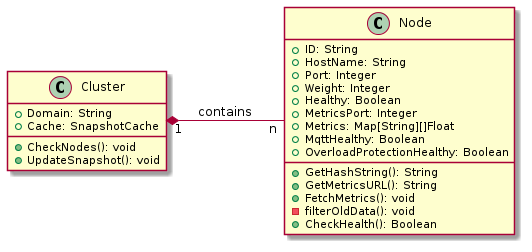
\includegraphics[scale=0.6]{gen/class.png}
    \caption{Die Abbildung zeigt das UML Klassendiagramm der entwickelten Control Plane.}
    \label{fig:class-diagram}
\end{figure}

\begin{comment}
\paragraph{Cluster}
In der \verb|main| Methode der Control Plane wird eine Cluster Struktur erstellt. Diese wird folgend an alle anderen Go Routinen übergeben, damit immer auf die aktuelle HiveMQ Cluster Topologie zugegriffen werden kann. Die Liste der HiveMQ Nodes in einer Cluster Struktur ist ein Golang Slice. Die Elemente dieses Slices werden niemals geändert. Falls sich die Topologie des HiveMQ Clusters ändert, wird ein neues Slice erstellt und in der Cluster Struktur referenziert. Sobald sich eine Go Routine das Slice eines Clusters in einer Variable speichert ist dadurch garantiert, dass sich die Werte dieses Slices nicht mehr ändern. Dies ist erforderlich, da es in Golang keine unveränderbare Listen gibt.

\paragraph{Node}
Eine HiveMQ Struktur repräsentiert ein HiveMQ Node und enthält alle Metadaten eines HiveMQ Nodes. Die Funktion \verb|NewHiveMQ| erstellt eine neue HiveMQ Struktur und gibt die Referenz auf diese zurück. Von HiveMQ Strukturen existieren nur Referenzen in der Control Plane. Dadurch können Werte der einzelnen Strukturen verändert werden ohne eine neue Struktur zu erstellen.
Eine HiveMQ Struktur besitzt eine Map mit einem String als Schlüssel und einer Liste aus Datenpunkten als Wert. In dieser Map werden die Metriken des HiveMQ Nodes abgespeichert. Der Schlüssel ist der jeweilige Prometheus Schlüssel der Metrik und die Liste der Datenpunkte ist nach Zeitstempel sortiert. Der erste Wert der Liste ist der älteste Wert. Damit die Control Plane nicht unendlich viel Arbeitsspeicher verbraucht indem sie alle Metriken für die gesamte Laufzeit abspeichert, werden Metriken, die älter als 60 Sekunden sind, gelöscht.

\paragraph{Resources}
Die Funktion \verb|GenerateSnapshot| aus dem Resources Namespace kriegt eine Liste von HiveMQ Strukturen übergeben. Aus dieser Liste wird in dieser Komponente die gesamte Envoy Konfiguration erstellt. Zunächst wird die Liste der Nodes nach ihrer ID sortiert damit eine Veränderung der Reihenfolge der Nodes keine Veränderung der Snapshotversion zur Folge hat. Nachdem alle Ressourcen entsprechend der HiveMQ Strukturdaten generiert wurden, wird eine Snapshot Version erstellt. Diese ist der Hash von \ac{ip} Adresse, Port, Health Status und Gewichtung eines jeden HiveMQ Nodes. Durch den Hash wird sichergestellt, dass eine Änderung von einer dieser Werte eine neue Version zur Folge hat. Au{\ss}erdem werden keine neuen Versionen erstellt, falls sich die Daten nicht ändern wodurch keine vermeintlich neuen Version an die Envoys ausgeliefert werden.

\paragraph{Metrics}
Die Metriken Komponente ruft bei Aufruf der \verb|InitMetrics| Funktion die aktuellen Metriken aller HiveMQ Nodes ab und startet zwei Go Routinen. Durch den initialen Abruf der Metriken werden alle Variablen initialisiert. Eine der beiden Go Routinen ist für das periodische Abrufen aller Metriken zuständig. Diese werden in der HiveMQ Struktur gespeichert. Die andere Go Routine verarbeitet periodisch die abgerufenen Metriken und berechnet die aktuelle Gewichtung und den Health Status. Diese Jobs wurden in zwei Go Routinen aufgeteilt um öfter die Metriken abzurufen als diese zu verarbeiten. Dies führt zu einer höheren Auflösung beim verarbeiten der Daten ohne alle zwei Sekunden die Envoy Konfiguration zu aktualisieren.

\paragraph{Main}
Die Main Komponente ist der Eintiegspunkt der Control Plane. Bei Aufruf wird zunächst eine Cluster Struktur erstellt, eine gegebene Domain aufgelöst und für alle \ac{ip} Adressen eine HiveMQ Struktur erstellt.
Anschlie{\ss}end werden zwei Go Routinen gestartet. Die erste löst periodisch den Domain Namen des Clusters auf um Topologieänderungen am Cluster umzusetzen. Die zweite Go Routine prüft periodisch die \ac{mqtt} Funktionalität eines jeden HiveMQ Nodes durch die Methode \verb|CheckHealth| der HiveMQ Struktur.
\end{comment}

\newpage
\subsection{Funktionalität}
\subsubsection{DNS Cluster Discovery}
Die \ac{dns} Cluster Discovery aus Kapitel \ref{ss:dns-discovery} ist in der Cluster Komponente implementiert.
Beim Start der Control Plane wird von der Main Komponente eine Go Routine gestartet, die periodisch und asynchron in einem gegebenen Intervall die Funktion \verb|CheckNodes| der Cluster Struktur aufruft. Diese verwendet die \verb|net| Standard Bibliothek von Golang, um den Domainnamen des Clusers aufzulösen und für alle \ac{ip} Adressen eine Node Struktur erstellt. Wenn bereits eine Node Struktur für ein \ac{ip} Adressen und Port Paar vorhanden ist, wird die Referenz der Struktur in die neue Liste übernommen.

\subsubsection{Weighted Round Robin}
Der weighted round-robin Algorithmus basierend auf der \ac{cpu} Auslastung der einzelnen HiveMQ Nodes aus Kapitel \ref{ss:weighted-cpu} ist in der Metrics Komponente implementiert.
\\
Quellcodeauszug \ref{code:weighted-cpu} zeigt den Algorithmus für die Bestimmung der Gewichtung der HiveMQ Nodes anhand der \ac{cpu} Auslastung.
Zeile 8 - 17 berechnen die durchschnittliche \ac{cpu} Auslastung aller gespeicherten Metriken individuell für jeden Node. Abgefragte Metriken werden nur für einen bestimmten Zeitraum gespeichert (siehe Kapitel \ref{si:control-plane}). Durch die Bildung des Durchschnittwertes über einen bestimmten Zeitraum, wird die Regelung der Gewichtung träge. Somit wird die Auswirkung von kurzfristigen Lastspitzen auf die Gewichtung reduziert.
Zeile 19 - 34 bestimmen die Gewichtung der Nodes basierend der zuvor berechneten Durchschnittsauslastung. Die Metrik der \ac{cpu} Auslastung kann einen Maximalwert von 100 erreichen. Da die freie \ac{cpu} Auslastung für die Gewichtung verwendet wird, wird die Durchschnittsauslastung von der maximalen Auslastung abgezogen, um die freie Auslastung zu erhalten. Bevor das Ergebnis als Gewichtung gesetzt wird, muss überprüft werden, ob dieses \verb|NaN| oder kleiner als eins ist, da dies die kleinste erlaubte Gewichtung in Envoy ist.
\begin{figure}
    \import{gen/}{weighted-cpu}
    \caption{Der Quellcodeauszug zeigt einen Algorithmus in Golang um die Gewichtungen von HiveMQ Nodes basierend ihrer CPU Auslastungen zu bestimmen.}
    \label{code:weighted-cpu}
\end{figure}

\subsubsection{Health Check} \label{si:health-check}
Der \ac{mqtt} Health Check aus Kapitel \ref{ss:health-check} ist in der Node Komponente implementiert. Die Funktion \verb|CheckHealth| wird periodisch für jeden HiveMQ Node in einer Go Routine der Main Komponente aufgerufen. Wenn die \verb|CheckHealth| Methode \verb|false| zurückgibt, ist der HiveMQ Node nicht in der Lage neue Client Verbindungen zu erhalten und sein Health Status wird auf \verb|UNHEALTHY| gesetzt. Es wird au{\ss}erdem sofort ein neuer Snapshot in den Cache geschrieben, damit so wenig Clients wie möglich mit einem \verb|UNHEALTHY| HiveMQ Node verbunden werden. Der \ac{mqtt} Health Status wird au{\ss}erdem in die Variable \verb|MqttHealthy| der Node Struktur gespeichert, damit diese von anderen Komponenten verarbeitet werden kann. Für den Fall, dass mehrere Faktoren den Health Status eines Nodes bestimmen, müssen alle Faktoren den Status \verb|HEALTHY| aufweisen damit ein Node derart gekennzeichnet wird.
\\
Eclipse stellt eine Open Source \ac{mqtt} Bibliothek für Golang bereit.
\cite{EclipsePahoMqtt2021}
Die Bibliothek bietet eine Abstraktion für das \ac{mqtt} Protokoll und übernimmt das de- und enkodieren von \ac{mqtt} Paketen. Die Funktion \verb|CheckHealth| wurde mit der Bibliothek programmiert und verhält sich wie das in Abbildung \ref{fig:health-check-sequence} dargestellte Ablaufdiagramm.

\subsubsection{Überlastschutz}
Der Überlastschutz aus Kapitel \ref{ss:circuit-breaking} ist in der Metrics Komponente implementiert. Quellcodeauszug \ref{code:circuit-breaking} zeigt den Algorithmus, um den Health Status aller Nodes basierend der Metrik \verb|OverloadProtection| zu bestimmen. In Zeile 10 wird auf den zuletzt bekannten Wert der Metrik zugegriffen und in Zeile 12 wird die Varible \verb|OverloadProtectionHealthy| der HiveMQ Struktur auf \verb|true| gesetzt, falls der Wert der Metrik kleiner oder gleich fünf ist.
Sobald der Overload Protection Wert überschritten wurde, oder der \ac{mqtt} Health Check aus Kapitel \ref{si:health-check} fehlgeschlagen ist, darf der HiveMQ Node nicht mehr als \verb|HEALTHY| gekennzeichnet werden. Zeile 18 - 22 setzen den Health Status erst auf \verb|HEALTHY| sobald beide Bedingungen erfüllt sind.
\begin{figure}
    \import{gen/}{circuit-breaking}
    \caption{Der Quellcodeauszug zeigt einen Algorithmus in Golang, der den Health Status eines HiveMQ Nodes basierend der Overload Protection Prometheus Metrik bestimmt.}
    \label{code:circuit-breaking}
\end{figure}
\newpage

\subsection{Einsatz}
In Kapitel \ref{ss:control-plane} wurde der Einsatz des Envoy \acl{lb} in einem \ac{mqtt} Anwendungsfeld bereits eingeordnet. Abbildung \ref{fig:deployment-diagram} zeigt den Aufbau einer HiveMQ Cluster Installation mit einem Envoy als \ac{lb} und einer Control Plane.
\\
\ac{mqtt} Clients bauen ihre Verbindung mit der Envoy Instanz auf, die das HiveMQ Cluster transparent zum Client abstrahiert. Die Envoy Instanz erhält seine Konfiguration von der Control Plane und entscheidet auf dessen Grundlagen, mit welchem HiveMQ Node ein neuer Client verbunden wird. Die Control Plane ruft periodisch die aktuellen Metriken aller HiveMQ Nodes des Clusters ab. Anhand der Metriken werden Health Status und Gewichtung der einzelnen Nodes bestimmt.
\begin{figure}
    \centering
    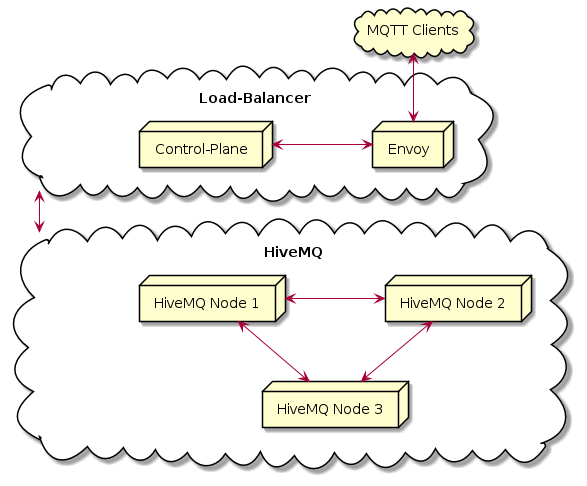
\includegraphics[scale=0.6]{gen/deployment.png}
    \caption{Die Abbildung zeigt das UML Einsatzdiagramm der in der vorliegenden Arbeit entwickelten Control Plane.}
    \label{fig:deployment-diagram}
\end{figure}
\\
Bei der in Abbildung \ref{fig:deployment-diagram} gezeigten Architektur müssen weder HiveMQ Nodes, noch Control Plane, für die \ac{mqtt} Clients erreichbar sein. Control Plane und Envoy müssen Netzwerkverbindungen mit allen Nodes des HiveMQ Clusters aufbauen können.
\\
Es können sich mehrere Envoy Instanzen bei einer Control Plane registrieren.
Um die einzelnen Envoy Instanzen für die \ac{mqtt} Clients zu abstrahieren, wird ihnen ein Cloud \acl{lb} vorgeschaltet.
Da jeder Envoy seine Konfiguration von der Control Plane erhält, wird in jeder Envoy Instanz dieselbe load balancing Entscheidung getroffen.
Eine solche Installation ist, wie ein HiveMQ Cluster, horizontal skalierbar.
\newpage
